\begin{figure}[H]
    \centering
    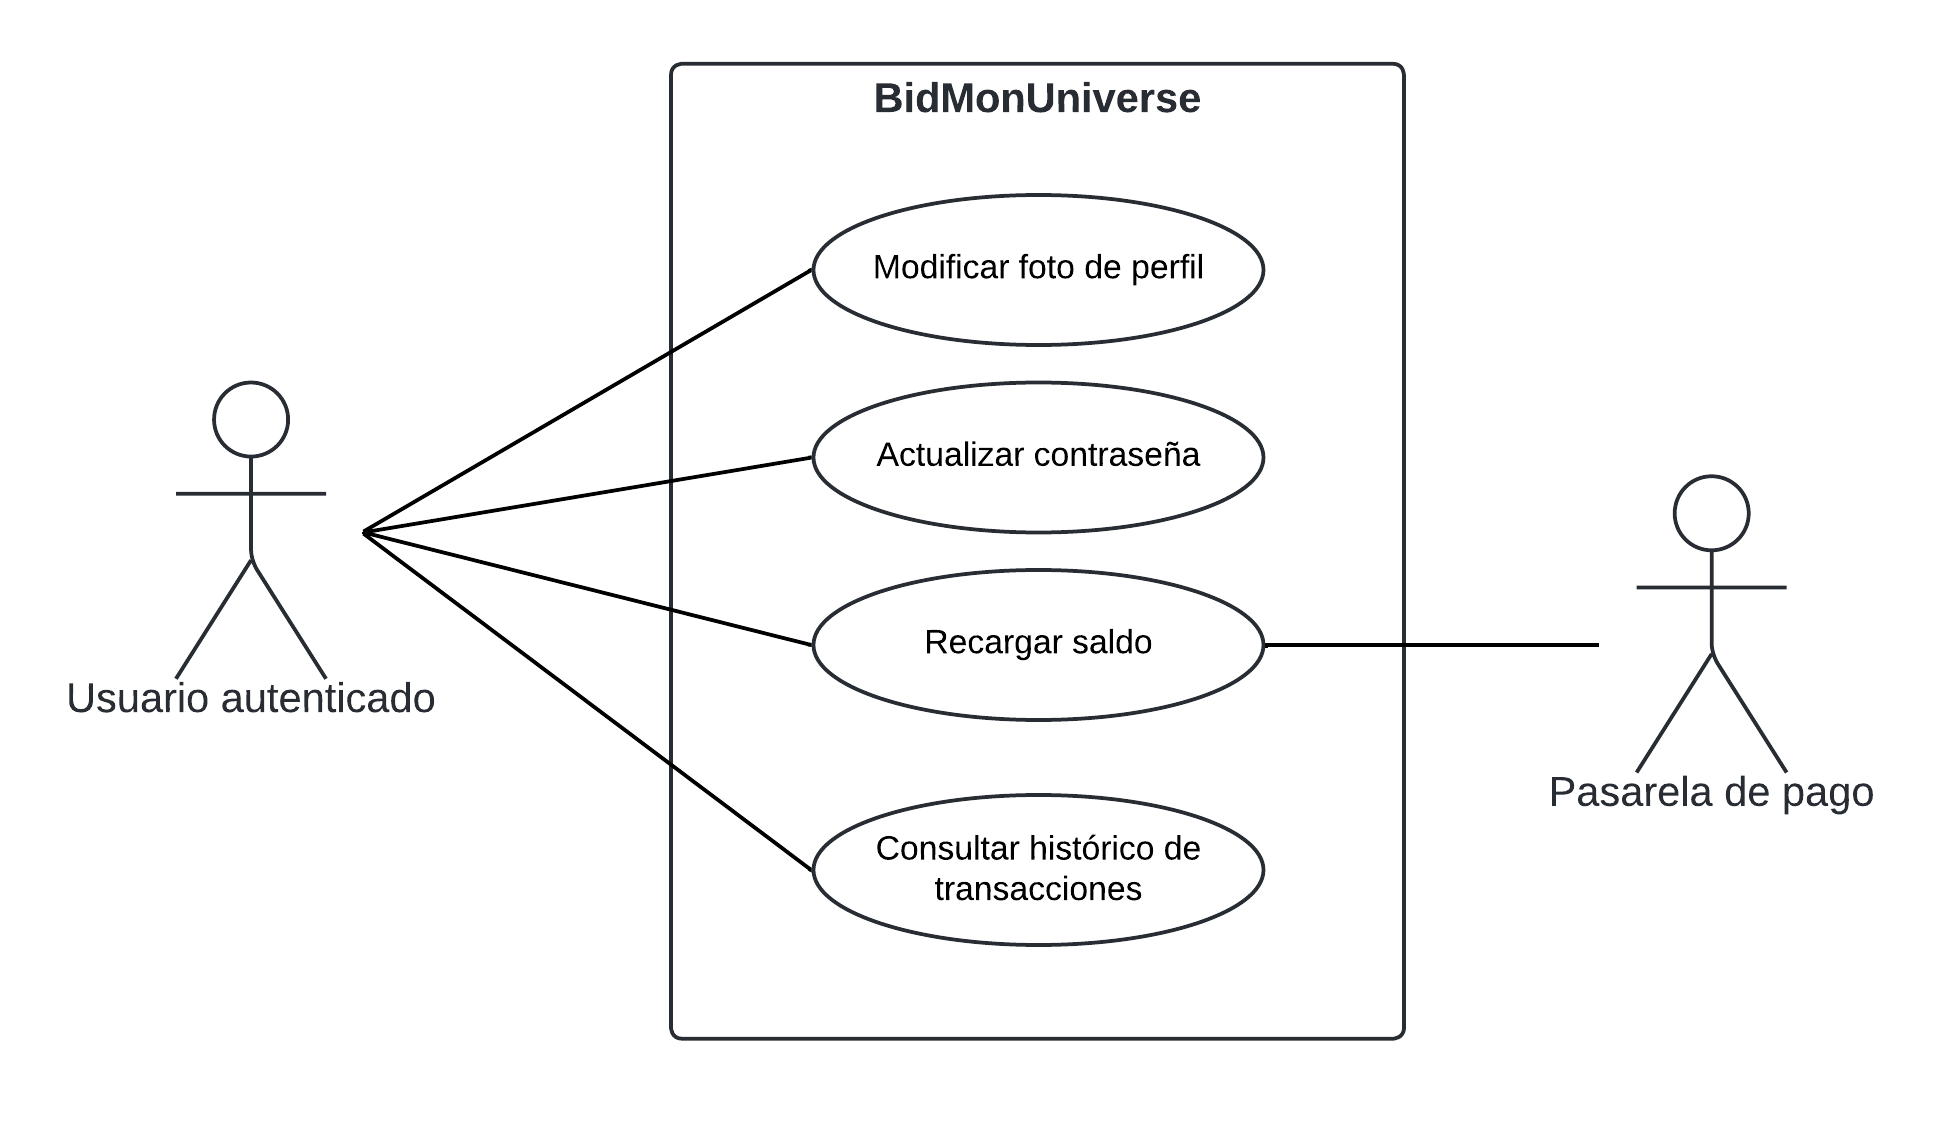
\includegraphics[width=0.5\textwidth]{figures/6-Analisis/6-Casos-uso/6_3_2_Gestion-perfil.png}
    \caption{Casos de uso. Gestión de perfil}
    \label{fig:cu_gestion-perfil}
\end{figure}
\subsubsection{Caso de uso. Modificar foto de perfil} \label{sec:cu_modificar-perfil}
\begin{longtable}{
    >{\columncolor{lightgreen!20}}p{4cm}
    p{12cm}
    }
    \caption{Caso de uso. Modificar foto de perfil} \label{table:cu_modificar-perfil} \\
    \toprule
    \rowcolor{darkgreen!50}
    \textbf{Caso de uso} & \multicolumn{1}{>{\columncolor{darkgreen!50}\centering\arraybackslash}p{12cm}}{\textbf{MODIFICAR PERFIL}} \\
    \endfirsthead
    
    \multicolumn{2}{c}%
    {{ \tablename\ \thetable{} Caso de uso. Modificar foto de perfil -- continuación de la página anterior}} \\
    \toprule
    \rowcolor{darkgreen!50}
    \textbf{Caso de uso} & \multicolumn{1}{>{\columncolor{darkgreen!50}\centering\arraybackslash}p{12cm}}{\textbf{MODIFICAR PERFIL}} \\
    \midrule
    \endhead
    
    \midrule
    \multicolumn{2}{r}{{Continúa en la siguiente página...}} \\ 
    \endfoot
    
    \bottomrule
    \endlastfoot
    
    \midrule
    Descripción & Un usuario autenticado puede modificar su foto de perfil de usuario. \\
    \midrule
    Actores principales & Usuario autenticado \\
    \midrule
    Actores secundarios &  \\
    \midrule
    Precondiciones & \begin{itemize}[nosep,leftmargin=*]
        \item El usuario debe haber iniciado sesión en el sistema.
    \end{itemize} \\
    \midrule
    Postcondiciones & \begin{itemize}[nosep,leftmargin=*]
        \item Se modifica el campo de la foto de perfil del usuario en la base de datos.
    \end{itemize} \\
    \midrule
    Disparadores & El usuario accede a la sección de modificar perfil. \\
    \midrule
    Escenario principal & \begin{enumerate}[nosep,leftmargin=*]
        \item El usuario accede a la sección de modificar perfil.
        \item El sistema muestra la opción de modificar la foto de perfil.
        \item El usuario hace clic en la opción de modificar la foto de perfil.
        \item El sistema muestra las imágenes predefinidas para que el usuario pueda seleccionar una.
        \item El usuario selecciona una imagen.
        \item El usuario hace clic en el botón de guardar.
        \item El sistema modifica el campo de la foto de perfil del usuario en la base de datos.
        \item El sistema muestra un mensaje de éxito.
        \item El sistema redirige al usuario a la página principal.
    \end{enumerate} \\
    \midrule
    Escenarios alternativos & 
    \begin{itemize}[nosep,leftmargin=*]
        \item \textbf{Escenario alternativo 1. El usuario cancela la modificación de perfil.}
        \begin{enumerate}[nosep,leftmargin=*]
            \item El usuario no hace clic en el botón de guardar.
            \item El sistema no modifica los datos del perfil del usuario.
        \end{enumerate}
    \end{itemize} \\
    \midrule
    Situaciones de error & 
    \begin{itemize}[nosep,leftmargin=*]
        \item \textbf{Error de conexión a la base de datos.}
        \begin{enumerate}[nosep,leftmargin=*]
            \item El sistema mostrará un mensaje de error.
            \item El sistema no modificará los datos del perfil del usuario.
        \end{enumerate}
    \end{itemize} \\
\end{longtable}


\subsubsection{Caso de uso. Actualizar contraseña} \label{sec:cu_actualizar-contrasena}
\begin{longtable}{
    >{\columncolor{lightgreen!20}}p{4cm}
    p{12cm}
    }
    \caption{Caso de uso. Actualizar contraseña} \label{table:cu_actualizar-contrasena} \\
    \toprule
    \rowcolor{darkgreen!50}
    \textbf{Caso de uso} & \multicolumn{1}{>{\columncolor{darkgreen!50}\centering\arraybackslash}p{12cm}}{\textbf{ACTUALIZAR CONTRASEÑA}} \\
    \endfirsthead
    
    \multicolumn{2}{c}%
    {{ \tablename\ \thetable{} Caso de uso. Actualizar contraseña -- continuación de la página anterior}} \\
    \toprule
    \rowcolor{darkgreen!50}
    \textbf{Caso de uso} & \multicolumn{1}{>{\columncolor{darkgreen!50}\centering\arraybackslash}p{12cm}}{\textbf{ACTUALIZAR CONTRASEÑA}} \\
    \midrule
    \endhead
    
    \midrule
    \multicolumn{2}{r}{{Continúa en la siguiente página...}} \\ 
    \endfoot
    
    \bottomrule
    \endlastfoot
    
    \midrule
    Descripción & Un usuario autenticado puede actualizar su contraseña de usuario. \\
    \midrule
    Actores principales & Usuario autenticado \\
    \midrule
    Actores secundarios &  \\
    \midrule
    Precondiciones & \begin{itemize}[nosep,leftmargin=*]
        \item El usuario debe haber iniciado sesión en el sistema.
    \end{itemize} \\
    \midrule
    Postcondiciones & \begin{itemize}[nosep,leftmargin=*]
        \item Se modifica la contraseña del usuario en la base de datos.
    \end{itemize} \\
    \midrule
    Disparadores & El usuario accede a la sección de modificar perfil. \\
    \midrule
    Escenario principal & \begin{enumerate}[nosep,leftmargin=*]
        \item El usuario accede a la sección de modificar perfil.
        \item El sistema muestra la opción de modificar la contraseña.
        \item El usuario hace clic en la opción de modificar la contraseña.
        \item El sistema muestra un formulario con los campos de la nueva contraseña y la confirmación de la nueva contraseña.
        \item El usuario completa los campos del formulario.
        \item El usuario hace clic en el botón de guardar.
        \item El sistema modifica el campo de la contraseña del usuario en la base de datos.
        \item El sistema muestra un mensaje de éxito.
        \item El sistema redirige al usuario a la página principal.
    \end{enumerate} \\
    \midrule
    Escenarios alternativos & 
    \begin{itemize}[nosep,leftmargin=*]
        \item \textbf{Escenario alternativo 1. El usuario cancela la modificación de perfil.}
        \begin{enumerate}[nosep,leftmargin=*]
            \item El usuario no hace clic en el botón de guardar.
            \item El sistema no modifica los datos del perfil del usuario.
        \end{enumerate}
        \item \textbf{Escenario alternativo 2. El usuario no completa correctamente los campos del formulario.}
        \begin{enumerate}[nosep,leftmargin=*]
            \item El usuario no completa correctamente los campos del formulario.
            \item El sistema muestra un mensaje de error.
            \item El sistema no modifica los datos del perfil del usuario.
        \end{enumerate}
    \end{itemize} \\
    \midrule
    Situaciones de error & 
    \begin{itemize}[nosep,leftmargin=*]
        \item \textbf{Error de conexión a la base de datos.}
        \begin{enumerate}[nosep,leftmargin=*]
            \item El sistema mostrará un mensaje de error.
            \item El sistema no modificará los datos del perfil del usuario.
        \end{enumerate}
    \end{itemize} \\
\end{longtable}




\subsubsection{Caso de uso. Recargar saldo} \label{sec:cu_recarga-saldo}
\begin{longtable}{
    >{\columncolor{lightgreen!20}}p{4cm}
    p{12cm}
    }
    \caption{Caso de uso. Recargar saldo} \label{table:cu_recarga-saldo} \\
    \toprule
    \rowcolor{darkgreen!50}
    \textbf{Caso de uso} & \multicolumn{1}{>{\columncolor{darkgreen!50}\centering\arraybackslash}p{12cm}}{\textbf{RECRAGAR SALDO}} \\
    \endfirsthead
    
    \multicolumn{2}{c}%
    {{ \tablename\ \thetable{} Caso de uso. Recargar saldo -- continuación de la página anterior}} \\
    \toprule
    \rowcolor{darkgreen!50}
    \textbf{Caso de uso} & \multicolumn{1}{>{\columncolor{darkgreen!50}\centering\arraybackslash}p{12cm}}{\textbf{RECARGAR SALDO}} \\
    \midrule
    \endhead
    
    \midrule
    \multicolumn{2}{r}{{Continúa en la siguiente página...}} \\ 
    \endfoot
    
    \bottomrule
    \endlastfoot
    
    \midrule
    Descripción & Un usuario autenticado puede recargar saldo en su cuenta. \\
    \midrule
    Actores principales & Usuario autenticado \\
    \midrule
    Actores secundarios &  Pasarela de pago \\
    \midrule
    Precondiciones & \begin{itemize}[nosep,leftmargin=*]
        \item El usuario debe haber iniciado sesión en el sistema.
    \end{itemize} \\
    \midrule
    Postcondiciones & \begin{itemize}[nosep,leftmargin=*]
        \item Se incrementa el saldo del usuario en la base de datos.
    \end{itemize} \\
    \midrule
    Disparadores & El usuario accede a la sección de recarga de saldo. \\
    \midrule
    Escenario principal & \begin{enumerate}[nosep,leftmargin=*]
        \item El sistema muestra el formulario de recarga de saldo.
        \item El usuario introduce la cantidad de saldo que desea recargar.
        \item El usuario hace clic en el botón de recargar saldo.
        \item El sistema valida la cantidad de saldo introducida.
        \item El sistema redirige al usuario a la pasarela de pago.
        \item El usuario completa el pago.
        \item El sistema incrementa el saldo del usuario en la base de datos.
        \item El sistema muestra un mensaje de éxito.
    \end{enumerate} \\
    \midrule
    Escenarios alternativos & 
    \begin{itemize}[nosep,leftmargin=*]
        \item \textbf{Escenario alternativo 1. El usuario cancela la recarga de saldo en la pasarela de pago.}
        \begin{enumerate}[nosep,leftmargin=*]
            \item El usuario cancela el pago.
            \item El sistema no incrementa el saldo del usuario en la base de datos.
            \item El sistema redirige al usuario a la página que muestra su saldo actual.
            \item El sistema muestra un mensaje de cancelación.
        \end{enumerate}
        \item \textbf{Escenario alternativo 2. El usuario introduce una cantidad de saldo inválida.}
        \begin{enumerate}[nosep,leftmargin=*]
            \item El sistema muestra un mensaje de error.
            \item El sistema muestra los campos con errores.
            \item El sistema permite al usuario corregir los errores.
        \end{enumerate}
    \end{itemize} \\
    \midrule
    Situaciones de error & 
    \begin{itemize}[nosep,leftmargin=*]
        \item \textbf{Error de conexión a la base de datos.}
        \begin{enumerate}[nosep,leftmargin=*]
            \item El sistema mostrará un mensaje de error.
            \item El sistema no incrementará el saldo del usuario en la base de datos.
            \item El sistema le dará al usuario la opción de intentar recargar de nuevo el saldo o volver a la página de inicio.
        \end{enumerate}
        \item \textbf{Error en la pasarela de pago.}
        \begin{enumerate}[nosep,leftmargin=*]
            \item El sistema mostrará un mensaje de error.
            \item El sistema no incrementará el saldo del usuario en la base de datos.
            \item El sistema redirigirá al usuario a la página de recarga de saldo.
        \end{enumerate}
    \end{itemize} \\
\end{longtable}

\subsubsection{Caso de uso. Histórico de transacciones realizadas} \label{sec:cu_transacciones-realizadas}
\begin{longtable}{
    >{\columncolor{lightgreen!20}}p{4cm}
    >{\columncolor{white}}p{12cm} 
    }
    \caption{Caso de uso. Histórico de transacciones realizadas} \label{table:cu_transacciones-realizadas} \\
    \toprule
    \rowcolor{darkgreen!50}
    \textbf{Caso de uso} & \multicolumn{1}{>{\columncolor{darkgreen!50}\centering\arraybackslash}p{12cm}}{\textbf{HISTÓRICO DE TRANSACCIONES REALIZADAS}} \\
    \endfirsthead
    
    \multicolumn{2}{c}%
    {{ \tablename\ \thetable{} Caso de uso. Histórico de transacciones realizadas -- continuación de la página anterior}} \\
    \toprule
    \rowcolor{darkgreen!50}
    \textbf{Caso de uso} & \multicolumn{1}{>{\columncolor{darkgreen!50}\centering\arraybackslash}p{12cm}}{\textbf{HISTÓRICO DE TRANSACCIONES REALIZADAS}} \\
    \midrule
    \endhead
    
    \midrule
    \multicolumn{2}{r}{{Continúa en la siguiente página...}} \\ 
    \endfoot
    
    \bottomrule
    \endlastfoot
    
    \midrule
    Descripción & Un usuario autenticado puede consultar el histórico de transacciones realizadas en el sistema. \\
    \midrule
    Actores principales & Usuario autenticado \\
    \midrule
    Actores secundarios &  \\
    \midrule
    Precondiciones & \begin{itemize}[nosep,leftmargin=*]
        \item El usuario debe haber iniciado sesión en el sistema.
    \end{itemize} \\
    \midrule
    Postcondiciones & \\
    \midrule
    Disparadores & El usuario accede a la sección de historial de transacciones. \\
    \midrule
    Escenario principal & \begin{enumerate}[nosep,leftmargin=*]
        \item El sistema muestra el historial de transacciones del usuario.
    \end{enumerate} \\
    \midrule
    Escenarios alternativos & 
    \begin{itemize}[nosep,leftmargin=*]
        \item \textbf{Escenario alternativo 1. El usuario no tiene transacciones realizadas.}
        \begin{enumerate}[nosep,leftmargin=*]
            \item El sistema mostrará un mensaje indicando que el usuario no tiene transacciones realizadas.
        \end{enumerate}
    \end{itemize} \\
    \midrule
    Situaciones de error & 
    \begin{itemize}[nosep,leftmargin=*]
        \item \textbf{Error de conexión a la base de datos.}
        \begin{enumerate}[nosep,leftmargin=*]
            \item El sistema mostrará un mensaje de error.
            \item El sistema le dará al usuario la opción de intentar cargar de nuevo el historial de transacciones o volver a la página principal.
        \end{enumerate}
    \end{itemize} \\
\end{longtable}